\documentclass[a4paper, 12pt, oneside]{article}

%---------------------------------------------------------------------------------
%------------------------- Set the variables for the Mainpage here ---------------
%---------------------------------------------------------------------------------
\newcommand{\name}{John Doe}
\newcommand{\email}{john@doe.com}
\newcommand{\osid}{OS-11111}

%---------------------------------------------------------------------------------
%------------------------- Include the list of used packages ---------------------
%---------------------------------------------------------------------------------
%Seitenränder definieren
\usepackage[right=4.0cm,left=3.3cm, bottom=3.9cm, top=4.1cm, footskip=2.1cm, headsep=2.0cm]{geometry}
\usepackage[utf8x]{inputenc}
\usepackage[T1]{fontenc}
\usepackage{palatino}
\linespread{1.25}
\usepackage{microtype}
\usepackage[english]{babel}
%More citations
\usepackage{natbib}
%better urls mit \url{}
\usepackage{url}
\usepackage{lastpage}
%code
\usepackage{listings}

%more colors
\usepackage{soul}

%Force figure to be placed “HERE”
\usepackage{float} 

%folgende Zeilen sind für Kapitelüberschriften
\usepackage[rigidchapters]{titlesec}
\usepackage{blindtext}
\titleformat{\chapter}
{\normalfont\LARGE}
{\makebox[3pc][l]{\LARGE\thechapter\hfil\rule[-6pt]{0.5pt}{2pc}}}
{0pt}
{\LARGE}
\titlespacing*{\chapter}{0pt}{0pt}{82pt}

%Csv -> Latex
\usepackage{csvsimple}

%Für Graphiken 
\usepackage{tikz}
\usetikzlibrary{plotmarks}
\usetikzlibrary{positioning,shapes,shadows,arrows}
\usepackage{graphicx}

%Paket gibt einige Optionen mehr bei Tabellen (wird eher nicht verwendet)
\usepackage{array}

%\usepackage{stdpage}
%test wegen anzahl zeilen pro seite
%Paket für Zeilenabstände
\usepackage{setspace}
%\onehalfspacing
\usepackage{multirow}
%Paket gibt mehr Kontrolle über die Captions (Bildunterschriften) bei Abbildungen
\usepackage[labelfont=bf,format=hang,font=footnotesize,justification=raggedright,singlelinecheck=false]{caption}

%Helvetia (Arial) Verwenden WICHTIG: Beide folgenden Zeilen kopieren!
%\usepackage[scaled]{helvet} %
%\renewcommand*\familydefault{\sfdefault} %%

% Abschalten des Einrückens bei neuen Absätzen (manuell, nach Tabellen, Abbildungen, etc.)
\setlength{\parindent}{0pt}
\hyphenation{}

% New Page before section
\newcommand{\sectionbreak}{\clearpage}

\usepackage{color}

\definecolor{color0}{rgb}{0,0,0}% black
\definecolor{color1}{rgb}{0.22,0.45,0.70}% light blue
\definecolor{color2}{rgb}{0.45,0.45,0.45}% dark grey
\definecolor{mygreen}{rgb}{0,0.6,0}
\definecolor{mygray}{rgb}{0.5,0.5,0.5}
\definecolor{myblue}{rgb}{0.0, 0.53, 0.74}
\definecolor{codebackground}{rgb}{0.8, 0.8, 0.8}
\definecolor{codechanged}{rgb}{0.8, 0.0, 0.0}

\lstset{ %
  backgroundcolor=\color{codebackground},   % choose the background color; you must add \usepackage{color} or \usepackage{xcolor}
  basicstyle=\footnotesize,        % the size of the fonts that are used for the code
  breakatwhitespace=false,         % sets if automatic breaks should only happen at whitespace
  breaklines=true,                 % sets automatic line breaking
  captionpos=b,                    % sets the caption-position to bottom
  commentstyle=\color{mygreen},    % comment style
  deletekeywords={...},            % if you want to delete keywords from the given language
  escapeinside={\%*}{*)},          % if you want to add LaTeX within your code
  extendedchars=true,              % lets you use non-ASCII characters; for 8-bits encodings only, does not work with UTF-8
% frame=single,	                   % adds a frame around the code
  keepspaces=true,                 % keeps spaces in text, useful for keeping indentation of code (possibly needs columns=flexible)
% keywordstyle=\color{blue},       % keyword style
% language=Octave,                 % the language of the code
% otherkeywords={*,...},           % if you want to add more keywords to the set
  numbers=left,                    % where to put the line-numbers; possible values are (none, left, right)
  numbersep=5pt,                   % how far the line-numbers are from the code
  numberstyle=\tiny\color{mygray}, % the style that is used for the line-numbers
  rulecolor=\color{black},         % if not set, the frame-color may be changed on line-breaks within not-black text (e.g. comments (green here))
  showspaces=false,                % show spaces everywhere adding particular underscores; it overrides 'showstringspaces'
  showstringspaces=false,          % underline spaces within strings only
  showtabs=false,                  % show tabs within strings adding particular underscores
  stepnumber=2,                    % the step between two line-numbers. If it's 1, each line will be numbered
% stringstyle=\color{mymauve},     % string literal style
  tabsize=2,	                   % sets default tabsize to 2 spaces
% title=\lstname,                   % show the filename of files included with \lstinputlisting; also try caption instead of title
  moredelim=**[is][\color{codechanged}]{**@}{@**}, %Rot für Änderungen
  moredelim=**[is][\color{myblue}]{***@}{@***}, %einfaches blau
  moredelim=**[is][\color{mygreen}]{*@}{@*},%einfaches Grün
}

%Aktives Inhaltsverzeichnis und links
\usepackage{hyperref}
\hypersetup{
    colorlinks,
    citecolor=black,
    filecolor=black,
    linkcolor=black,
    urlcolor=black
}

\usepackage{fancyhdr}
\pagestyle{fancy}
\fancypagestyle{plain}{}
\fancyhf{}
\fancyfoot{} % clear all footer fields

\fancyhead[R]{\small{\leftmark}}
\fancyhead[L]{\small{Offensive Security - Penetration Test Report}}
\renewcommand{\sectionmark}[1]{\markboth{#1}{}}

\renewcommand{\footrulewidth}{0.1pt} % Create a rule above the page number
\fancyfoot[R]{\textcolor{color1}\thepage  \textcolor{color2}{/\pageref{LastPage}}}

%---------------------------------------------------------------------------------
%------------------------- Create title page -------------------------------------
%---------------------------------------------------------------------------------
\title{{\textbf{\Huge Offensive Security}}\\ Penetration Test Report for\\Internal Lab and Exam}
\author{\vspace{3cm}\\{\LARGE \name}\\[1em]\email\\[1em]OSID: \osid}
\date{\vspace{7cm}\today}


\begin{document}
%---------------------------------------------------------------------------------
%------------------------- Print title page --------------------------------------
%---------------------------------------------------------------------------------
\maketitle
\thispagestyle{empty}
%---------------------------------------------------------------------------------
%------------------------- Print table of contents -------------------------------
%---------------------------------------------------------------------------------
% Attention: Document might need some runs to get all indexes etc right .. usual LaTeX stuff :)
\tableofcontents
\thispagestyle{empty}
\pagebreak

%---------------------------------------------------------------------------------
%------------------------- Declaring the empty variables for the hosts -----------
%---------------------------------------------------------------------------------
\newcommand{\hostname}{}
\newcommand{\ip}{}
\newcommand{\tcpports}{} 
\newcommand{\udpports}{} 
\newcommand{\os}{}
\newcommand{\vuln}{}
\newcommand{\product}{}
\newcommand{\vulnx}{}
\newcommand{\productx}{}

%---------------------------------------------------------------------------------
%------------ Here are the hosts, ------------------------------------------------
%------------ just add in the same scheme after you coppied the example folder ---
%---------------------------------------------------------------------------------
% !TeX spellcheck = en_US

%---------------------------------------------------------------------------------
%--------------------------Set the variables for every client---------------------
%---------------------------------------------------------------------------------
\renewcommand{\hostname}{Example}
\renewcommand{\os}{Linux OS Soft XP}
\renewcommand{\ip}{42.42.42.42}
\renewcommand{\tcpports}{1,2,3}
\renewcommand{\udpports}{23,42}
\renewcommand{\vuln}{CVE-123-42 \glqq Stupid Idiot User\grqq}
\renewcommand{\product}{Human}
%The x-Variables are only used, when root is defined (== root shell)
\renewcommand{\vulnx}{CVE-123-43 \glqq Very Stupid Idiot User Again\grqq} 
\renewcommand{\productx}{Human}
%%%Did you get root? Comment out if you only got low priv access
\def\gotroot{}   %%% Define root if you got root shell
%\undef\gotroot % Else undefine


%----------------------------------------------------------------------------------
%-------------------------------Auto generated content-----------------------------
%----------------------------------------------------------------------------------

\section{\hostname}
\subsection{Service Enumeration}

\begin{table}[h]
	\begin{tabular}{|c|c|}
		\hline
		\multicolumn{2}{|c|}{\textbf{\hostname}}\\\hline\hline
		Type         & Open ports   \\\hline
		TCP          & \tcpports{}  \\\hline
		UDP          & \udpports{}  \\\hline\hline
		\textbf{\os} & \textbf{\ip} \\\hline
	\end{tabular}
	\caption{Service enumeration \hostname}
\end{table}

\subsection{Remote Access Exploitation}

\paragraph{Vulnerability Exploited:}
\vuln

%----------------------------------------------------------------------------------
%-------------------------------Start writing here---------------------------------
%----------------------------------------------------------------------------------
 
\paragraph{Vulnerability Explanation:}
% You can answer the following questions:
% What is the problem?
% What can an attacker do with this vulnerability?
% How did you notice this bug?
% Did you need to change an exploit in order to run it?
% What was the result of the execution?


\paragraph{Vulnerability Fix:}
The publishers of \product{} have issued a patch to fix this known issue.

\paragraph{Severity:}
\textbf{\textcolor{red}{Critical}}

\paragraph{Proof of Concept:} 
Modifications to the existing exploit was needed and is highlighted in red.
\begin{lstlisting}[caption={Exploitation of \hostname}]
SELECT * FROM login WHERE id = **@1 or 1=1@** AND user LIKE "%root%"

if (x = y):
    space indent
	tab indent

In the code section :
*@Green Text@*
**@Red Text@**
***@Blue Text@***
\end{lstlisting}

\begin{figure}[H]
	\centering
	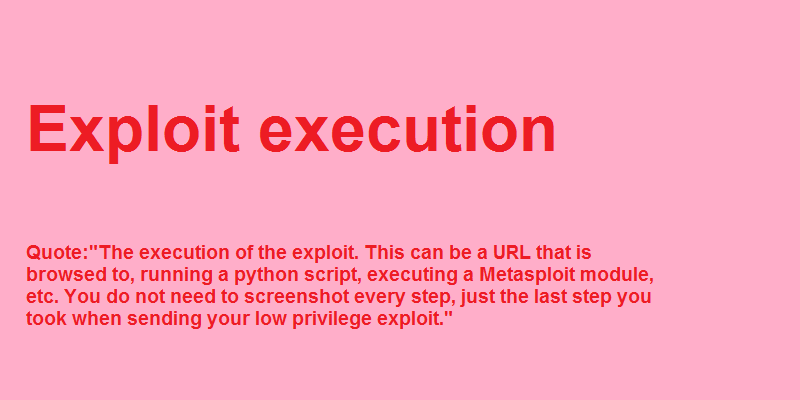
\includegraphics [width=1.0\textwidth]{./hosts/\hostname/1-remote-exploit.png}
	%scale 0.5 bedeutet 50% der originalgröße
	%angle=90 Grafik um 90° drehen
	\caption{Exploitation of \hostname}
\end{figure}

\paragraph{Proof of remote access:} %Print proof for local exploit here
The remote access can be proven with the following command:
\begin{lstlisting}[caption={Post exploitation of \hostname{} with low privileges}]
hostname && id && ifconfig && cat local.txt
\end{lstlisting}
\begin{figure}[H]
	\centering
	
\includegraphics [width=\textwidth]{./hosts/\hostname/2-local.png}
	\caption{Proof of remote access to \hostname}
\end{figure}

%----------------------------------------------------------------------------------
%------------------------------Conditional Privilege Escalation Block--------------
%----------------------------------------------------------------------------------
\ifdefined\gotroot

%----------------------------------------------------------------------------------
%------------------------------Part for Priv escalation----------------------------
%----------------------------------------------------------------------------------
\subsection{Privilege Escalation}

\paragraph{Vulnerability Exploited:}
\vulnx

\paragraph{Vulnerability Explanation:}
% You can answer the following questions:
% What is the problem?
% What can an attacker do with this vulnerability?
% How did you notice this bug?
% Did you need to change an exploit in order to run it?
% What was the result of the execution?


\paragraph{Vulnerability Fix:}
The publishers of \product{} have issued a patch to fix this known issue.

\paragraph{Severity:}
\textbf{\textcolor{red}{Critical}}

\paragraph{Proof of Concept:} 
Modifications to the existing exploit was needed and is highlighted in red.
\begin{lstlisting}[caption={Exploitation of \hostname}]
SELECT * FROM login WHERE id = **@1 or 1=1@** AND user LIKE "%root%"
In the code section :
*@Green Text@*
**@Red Text@**
***@Blue Text@***
\end{lstlisting}

\begin{figure}[H]
	\centering
	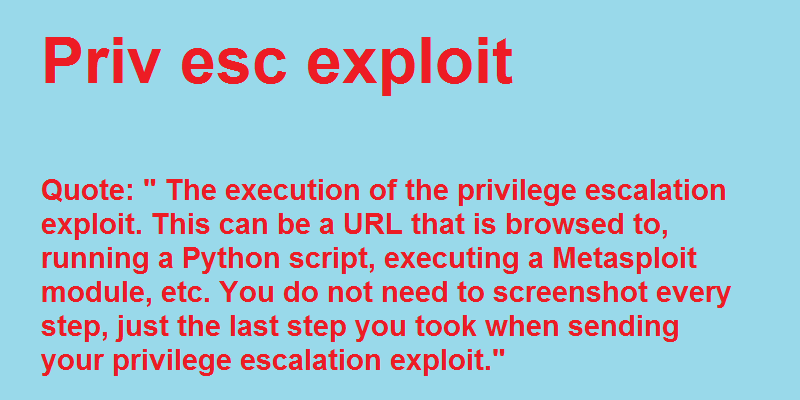
\includegraphics [width=1.0\textwidth]{./hosts/\hostname/3-privesc-exploit.png}
	\caption{Privilege escalation exploit of \hostname}
\end{figure}

\paragraph{Proof of successful privilege escalation:}
The successful privilege escalation can be proven with the following command:
\begin{lstlisting}[caption={Post exploitation of \hostname}]
hostname && id && ifconfig && cat proof.txt
\end{lstlisting}

\begin{figure}[H]
	\centering
	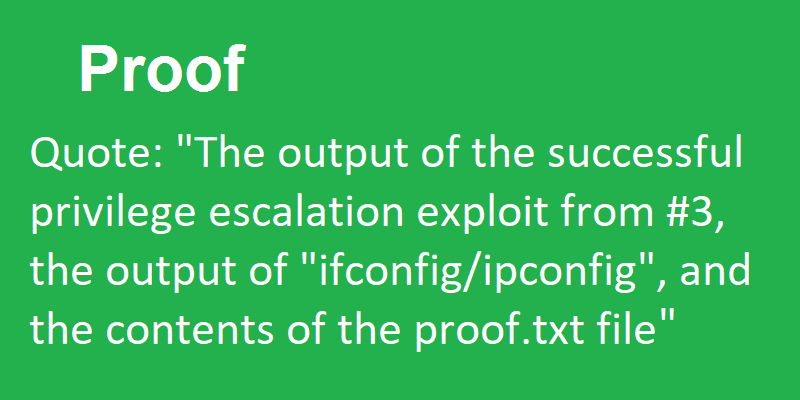
\includegraphics [width=\textwidth]{./hosts/\hostname/4-proof.png}
	\caption{Proof of successful privilege escalation on \hostname}
\end{figure}
\fi % End of if-block
%----------------------------------------------------------------------------------
%--------------------------------------End of Priv Esc Block-----------------------
%----------------------------------------------------------------------------------



\renewcommand{\hostname}{DeepThought}
\renewcommand{\os}{Earth}
\renewcommand{\ip}{42.42.42.23}
\renewcommand{\tcpports}{1,2,3}
\renewcommand{\udpports}{23,42}
\renewcommand{\vuln}{Vogons}
%Just choose one , comment out the other
\toggletrue{priv}
%\togglefalse{priv}

%--------------------------------------------------------------------------------------------------------------------
 
%---------------------------------------Start writing here-------------------------
\subsection{\hostname}
\subsubsection{Enumeration}

	\label{tab:\hostname}
\begin{longtable}{|c|c|}
\caption{Service enumeration \hostname}\\
\hline
\multicolumn{2}{|c|}{\textbf{\hostname}}\\
\hline
\hline
Type&open ports\\
\hline
TCP&\tcpports{}\\
\hline
UDP&\udpports{}\\

\hline
\hline
\multicolumn{1}{|c|}{\textbf{\os}}&\multicolumn{1}{|c|}{\textbf{\ip}}\\
\hline


\end{longtable}
\subsubsection{Exploitation}

\textit{Used Vulnerability: \vuln}\\

\textit{Vulnerability Explanation:}\\

BLA BLA WRITE SOMETHING HERE 


%please insert also the priv esc. cmmands in this block. Right now the files don't work as intended. If you need you can use also the post block .. just the if clause for the images don't like the code enviroment.
\begin{lstlisting}[caption={Exploitation of \hostname},label=\hostname-exploit]
*@Kali prep:@*

*@Modifications in the exploit@*
PANIC **@PANIC@** PANIC
*@Running the exploit@*

*@Escaping the low priv shell:@*
\end{lstlisting}


\begin{figure}[h!]
\centering
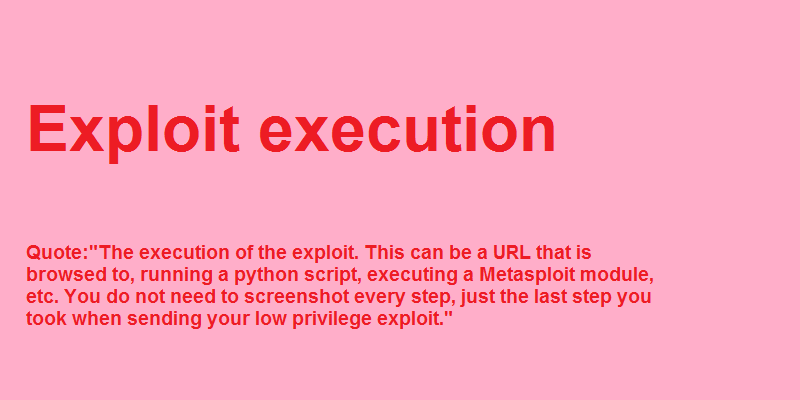
\includegraphics [width=\textwidth]{./hosts/\hostname/exploitexecution.png}
%scale 0.5 bedeutet 50% der originalgröße
%angle=90 Grafik um 90° drehen
\caption[Exploitation of \hostname]{Exploitation of \hostname} \label{\hostname-1}
\end{figure}


  \iftoggle{priv}
    {
   

%Conditional Privilege Escalation Block .. --------------------------------------------------------------------------------------------------------------------

\FloatBarrier

%Part for Priv escalation -------------------------------------------------------------------------------------------
\subsubsection{Privilege Escalation}




\begin{figure}[h!]
\centering

\includegraphics [width=\textwidth]{./hosts/\hostname/local.png}
%scale 0.5 bedeutet 50% der originalgröße
%angle=90 Grafik um 90° drehen
\caption[Local shell of \hostname]{Local shell of \hostname} \label{\hostname-2}
\end{figure}


\begin{figure}[h!]
\centering
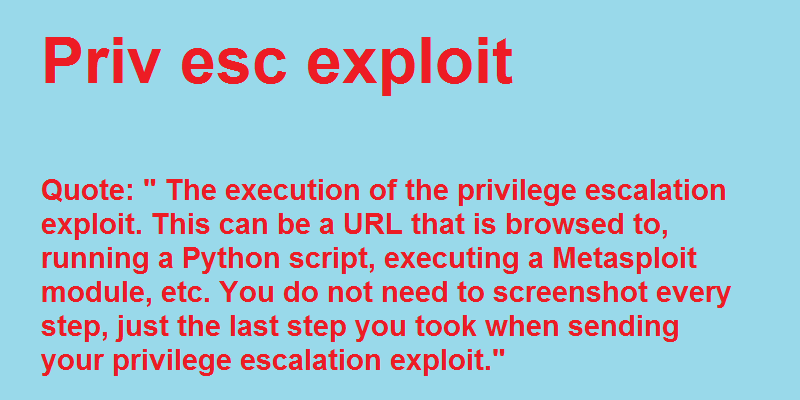
\includegraphics [width=\textwidth]{./hosts/\hostname/privescexploit.png}
%scale 0.5 bedeutet 50% der originalgröße
%angle=90 Grafik um 90° drehen
\caption[Priv escalation exploit of \hostname]{Priv escalation exploit of \hostname} \label{\hostname-3}
\end{figure}

}
{}
%--------------------------------------End of Priv Esc Block------------------------
\FloatBarrier
\subsubsection{Proof and Post escalation}
\begin{lstlisting}[caption={Post exploitation of \hostname},label=\hostname-post]
*@Post exploitation commands run:@*

\end{lstlisting}

\begin{figure}[h!]
\centering
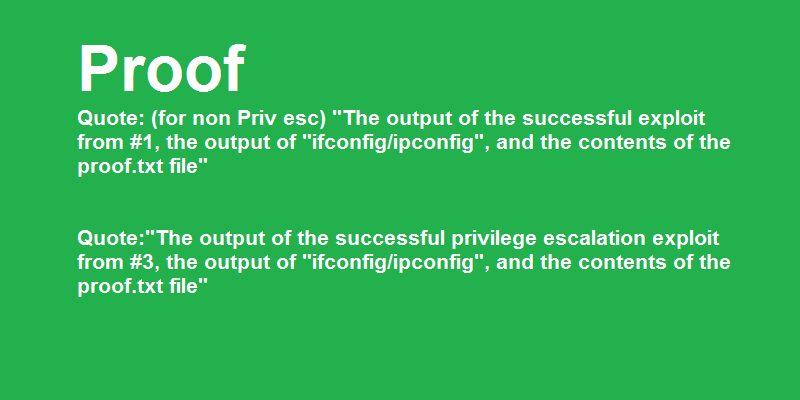
\includegraphics [width=\textwidth]{./hosts/\hostname/proof.png}
%scale 0.5 bedeutet 50% der originalgröße
%angle=90 Grafik um 90° drehen
\caption[Proof of \hostname]{Proof of \hostname} \label{\hostname-4}
\end{figure}


%---------------------End of host file


\end{document}
